\section{Lecture 2. Deterministic Discrete-Time System and Shortest Path Problems}
\subsection{Deterministic Finite-State DP Problems}
\centerline{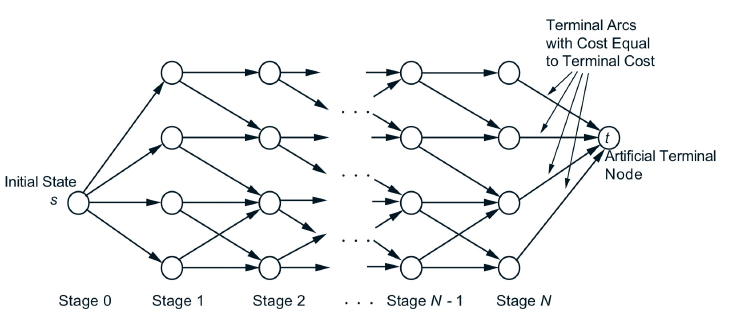
\includegraphics[width=12cm]{Lecture2/Fig1.png}}
\begin{itemize}
    \item Two conditions required for the transformation to the shortest path problem
    \begin{itemize}
        \item Deterministic
        \item Finite-state
    \end{itemize}
    A deterministic finite-state problem is equivalent to finding a shortest path from $s$ (initial state) to $t$ (terminal state)
    \item States: Nodes
    \item Controls: Arcs
    \item Control sequences (Open-loop): paths from initial state to terminal state
    \item $a_{ij}^k$: cost of transition from state $i\in S_k$ to state $j\in S_{k+1}$ at stage $k$ ("length" of the arc)
    \item $a_{it}^N$: terminal cost of state $i\in S_N$
    \item Cost of control sequence: cost of the corresponding path ("length" of the path)
\end{itemize}

\subsection{Backward and Forward DP Algorithm}
\begin{itemize}
    \item DP algorithm
    \begin{itemize}
        \item $J_N(i) = a_{it}^N,\quad i\in S_N$
        \item $J_k(i) = \min_{j\in S_{k+1}}[a_{ij}^k+J_{k+1}(j)],\quad i\in S_k,\quad k = 0,...,N-1$
    \end{itemize}
    The optimal cost is $J_0(s)$ and is equal to the length of the shortest path from $s$ to $t$
    \item Observation: An optimal path $s\to t$ is also an optimal path $t\to s$ in a "reverse" shortest path problem where the direction of each arc is reversed and its length is left unchanged
    \item In this situation: forward DP algorithm = backward DP algorithm
    \item For the reverse problem: 
    \begin{itemize}
        \item $\tilde{J}_N(i) = a_{it}^0,\quad i\in S_1$
        \item $\tilde{J}_k(i) = \min_{j\in S_{N-k}}[a_{ij}^{N-k}+\tilde{J}_{k+1}(i)],\quad i\in S_{N-k+1},\quad k = 1,...,N$
    \end{itemize}
    The optimal cost is $\tilde{J}_0(t) = \min_{i\in S_N} [a_{it}^N + \tilde{J}_1(i)]$
    \item View $\tilde{J}_k(j)$ as optimal-to-arrive to state $j$ from initial state $s$
\end{itemize}

\subsection{Note on Forward DP algorithms}
\begin{itemize}
    \item There is no Forward DP Algorithm for \textbf{stochastic} problems
    \item Mathmatically, for stochastic problems, we cannot restrict ourselves to open loop sequences, so the shortest path viewpoint fails
    \item Conceptually, in the presence of uncertainty the concept of "optimal cost-to-arrive" at a state $s_k$ does not make sence. It may be impossible to guarantee (with prob. 1) that any given state can be reached.
    \item By contrast, even in stochastic problems, the concept "optimal cost-to-go" from any state $s_k$ makes clear sense.
\end{itemize}

\subsection{Generic Shortest Path Problems}
\begin{itemize}
    \item $\{1,2,...,N,t\}$: Nodes of a graph ($t$: the destination)
    \item $a_{ij}$: cost of moving from node $i$ to node $j$
    \item Find a shortest (minimum cost) path from each node $i$ to node $t$
    \item Assumption: all cycles have nonnegative length. Then an optimal path need not take more than $N$ moves.\\
    \emph{Some arcs are allowed to have nagative length}
    \item We formulate the problem as one where we require exactly $N$ moves but allows degenerate moves from a node $i$ to itself with cost $a_{ii}=0$
    \begin{itemize}
        \item $J_k(i)$: optimal cost of getting from $i$ to $t$ in $N-k$ moves
        \item $J_0(i)$: cost of the optimal path from $i$ to $t$
    \end{itemize}
    \item DP algorithm:
    \begin{itemize}
        \item $J_k(i) = \min_{j=1,...,N}[a_{ij}+J_{k+1}(j)],\quad k = 0,...,N-2$
        \item $J_{N-1}(i) = a_{it},\quad i=1,2,...,N$
    \end{itemize}
\end{itemize}

\subsection{Example for Generic Shortest Path Problem}
At most 4 moves to the destination \\
\centerline{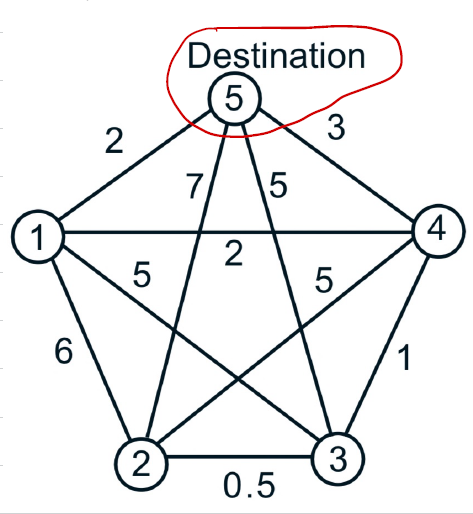
\includegraphics[width=8cm]{Lecture2/Fig2.png}}

Convert to equivalent staged-shortest-path-problem

\centerline{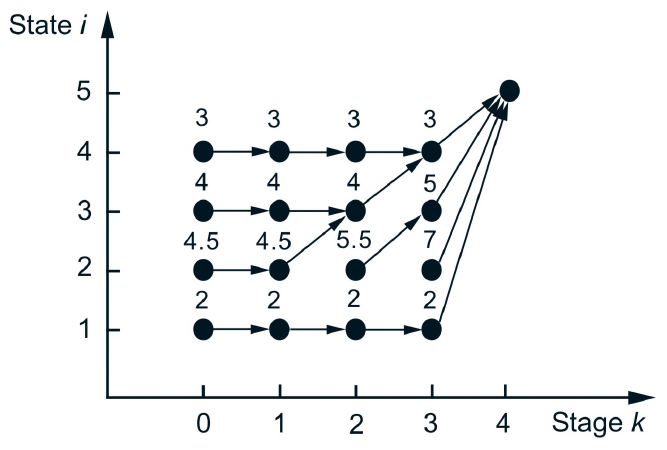
\includegraphics[width=10cm]{Lecture2/Fig3.png}}
\centerline{Bellman-Ford Algorithm}

\subsection{Critical Path Analysis}
[To be completed ...]

\subsection{Estimation/Hidden Markov Models}
\begin{itemize}
    \item Markov chain with transition probabilities $p_{ij}$
    \item State transitions are hidden from view
    \item For each trasition, we get an (independent) observation
    \item $r(z;i,j)$: Prob. the observation take value $z$ when the state transition is from $i$ to $j$
    \item \textbf{Trajectory estimation problem}: Given the observation sequence $Z_N=\{z_1,z_2,...,z_N\}$, what is the "most likely" state transition sequence $\hat{X}_N=\{\hat{x}_0,\hat{x}_1,...,\hat{x}_N\}$
    [one that maximizes $p(X_N|Z_N)$ over all $X_N=\{x_0,x_1,...,x_N\}$]
\end{itemize}

\subsection{Viterbi Algorithm}
Assumption of independent observation: an observation only depends on its corresponding transition
\begin{itemize}
    \item We have
    \[
        p(X_N|Z_N) = \frac{p(X_N,Z_N)}{p(Z_N)}
    \]
    where $p(X_N,Z_N)$ and $p(Z_N)$ are the unconditional probabilities of occurrance of $(X_N,Z_N)$ and $Z_N$
    \item Maximizing $p(X_N|Z_N)$ is equivalent with maximizing $\ln (p(X_N,Z_N))$
    \item We have
    \[
        \begin{array}{ll}
            p(X_N,Z_N)  & = p(x_0,x_1,...,x_N,z_1,z_2,...,z_N)  \\
                        & = \pi_{x_0}p(x_1,...,x_N,z_1,z_2,...,z_N|x_0) \\
                        & = \pi_{x_0}p(x_1,z_1|x_0)p(x_2,...,x_N,z_2,...,z_N|x_0,x_1,z_1) \\
                        & = \pi_{x_0}p_{x_0 x_1}r(z_1;x_0,x_1)p(x_2,...,x_N,z_2,...,z_N|x_0,x_1,z_1)^\dagger \\
                        & = \cdots \\
                        & = \pi_{x_0} \prod _{k=1}^N p_{x_{k-1}x_k} r(z_k;x_{k-1},x_k) 
        \end{array}
    \]
    so the problem is equivalent to 
    \[
        \min -\ln (\pi_{x_0}) - \sum_{k=1}^N \ln (p_{x_{k-1}x_k} r(z_k;x_{k-1},x_k))
    \]
    over all possible sequences $\{x_0,x_1,...,x_N\}$ \\
    $^\dagger$: The calculation can be continued by writing
    \[
        \begin{array}{ll}
            p(x_2,...,x_N,z_2,...,z_N|x_0,x_1,z_1) & = p(x_2,z_2 | x_0,x_1,z_1)p(x_3,...,x_N,z_3,...,z_N|x_0,x_1,z_1,x_2,z_2) \\
            & =p_{x_1x_2} r(z_2;x_1,x_2) p(x_3,...,x_N,z_3,...,z_N|x_0,x_1,z_1,x_2,z_2)^\ddagger \\

        \end{array}
    \]
    $^\ddagger$:
    \begin{itemize}
        \item $P(x_2|x_0,x_1,z_1)=P(x_2,x_1)$: Markov Property
        \item $P(z_2|x_1,x_2)=P(z_2|x_0,x_1,x_2,z_1)$: Independenc pf observation
    \end{itemize}
    \item This is a shortest path problem
\end{itemize}

\subsection{Advantage of Forward Alogrithm (for Viterbi Algorithm)}
\centerline{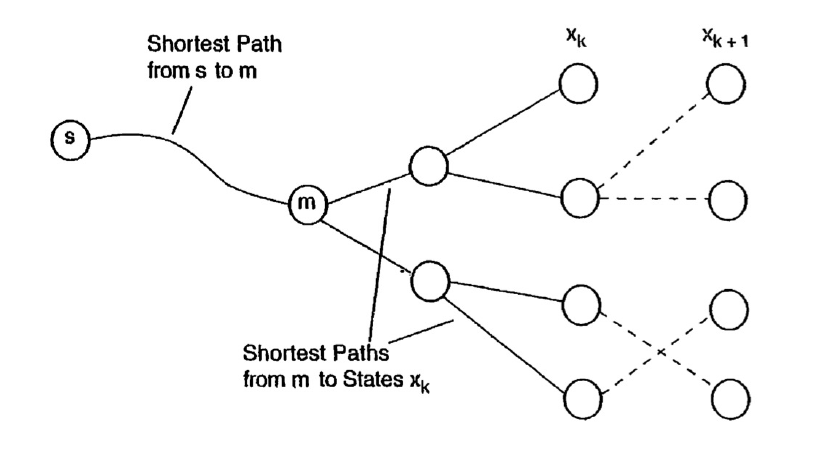
\includegraphics[width=15cm]{Lecture2/Fig4.png}}
Suppose that the shortest paths from $s$ to all states $x_k$ pass through a single node $m$. If an additional observation is received, the shortest 
paths from $s$ to all states $x_{k+1}$ will continue pass through $m$. Therefore, the portion of the state sequence up to node $m$ can be safely estimated because 
additional observations will not change the initial portion of the shortest paths from $s$ up to $m$. 

Thereofre, we can estimate a portion of state sequence \textbf{without waiting} to receive the entire observation sequence $Z_N$ for a number of practical schemes.

This is useful is $Z_N$ is a long sequence.

\subsection{General Shortest Path Algorithm}
\begin{itemize}
    \item There are many nonDP shortest path algorithms. They ca all be used to solve deterministic finite-state problems
    \item They may be preferable than DP if they avoid calculating the optimal cost-to-go of \textbf{EVERY} state
    \item This is essential for problems with \textbf{HUGE} state spaces. Such problems arise for example in combinatorial optimization
    \item Example: Traveling Salesman Problem (TSP)
\end{itemize}

\subsection{Traveling Salesman Problem}:
Find the shortest route that starts from Home City $o$, visits every other city $1,2,...,N$ exactly once and returns to Home City $o$
\begin{itemize}
    \item State: $(i,S)$. Now at city $i$, and still have to visit cities in $S$ and return to home city $o$
    \item Control: $j$. Which city should be visited next.
    \item System Dynamic: $(i,s)\stackrel{\text{\rm Control: }j}{\longrightarrow} (k,S\backslash \{j\})$
    \item Stage cost: $d_{ij}$. Distance from $i$ to $j$.
    \begin{itemize}
        \item $J_N(i,\emptyset)=d_{i,o}$
        \item $J_k(i,S)=\min_{i\in S} \{ d_{i,j} + J_{k+1}(j,S\backslash \{j\}) \} ^\dagger$
        \item $J_0(0,\{1,2,...,N\})$ gives the shortest tour.
    \end{itemize}
    \item Mehotds comparison
    \begin{itemize}
        \item Brute Force: $N!$
        \item DP: $N^2\cdot 2^N$. much less than $N!$
    \end{itemize}
\end{itemize}
$^\dagger$: Take $N$ evaluations for each pair of $(i,S)$. There are $N$ cities and $2^N$ subsets $S$ and $N$ stages. Total: $N\cdot N \cdot 2^N$

\subsection{Knapsack Problem}
\[
    \begin{array}{rl}
        \max & \sum_{i=1}^N v_i\cdot u_i \\
        \text{s.t.}  & \sum_{i=1}^N w_i\cdot u_i \leq W \text{ \rm (Integer)} \\
        & u_i \in \{0,1\},\quad \forall i=1,...,N        
    \end{array}
\]
\begin{itemize}
    \item Stage $k$: Items $1,...,k$ have been considered
    \item Stage $x_k$: The remaining capacity after considering items $1,...,k-1$. $x_k\in\{0,1,2,...,W\}$
    \item Control $u_k$: Whether to take item $k$. $u_k\in \{0,1\}$
    \item Stage Cost: $v_k\cdot u_k$
    \item System Dynamics: $x_{k+1}=x_k-w_k\cdot u_k$
    \item DP Algorithm:
    \begin{itemize}
        \item $
            J_k(x_k) = \left\{ \begin{array}{ll}
                J_{k+1}(x_k) & \text{\rm if } x_k < w_k \\
                \max \{ J_{k+1}(x_k), v_k+J_{k+1}(x_k-w_k) \} & \text{\rm if } x_k \geq w_k
            \end{array} \right. ,\quad 1\leq k\leq N-1$
        \item $
            J_N(x_N) = \left\{ \begin{array}{ll}
                0 & \text{\rm if } x_k < w_k \\
                v_N & \text{\rm if } x_k \geq w_k
            \end{array} \right.$
    \end{itemize}
    \item Computational Complexity: $O(N\cdot W)$, Pseudo-Polynomial. \\
    For each stage $k$ and each state $x_k$, at most $2$ operations. There are $N$ stages and $W+1$ possible states for every stage. \\
    $\Longrightarrow$ Total complexity: $O(N\cdot W)$
\end{itemize}

\subsection{Label Correcting Methods}
\begin{itemize}
    \item Given: origin $s$, destination $t$, lengths $a_{ij}\geq 0$
    \item Idea is to progressively discover shorter paths from the origin $s$ to every other node $i$
    \item Notation
    \begin{itemize}
        \item $d_i$ (label of $i$): length of the shortest path found (initially $d_s=0$, $d_i=\infty$ for $i\neq s$)
        \item UPPER: the label $d_t$ of the destination
        \item OPEN list: contains  nodes that are currently active in the sense that they are candidates for further examination (initially OPEN=$\{s\}$)
    \end{itemize}
\end{itemize}
Lable Correcting Algorithm
\begin{itemize}
    \item Step 1 (Node Removal): Remove a node $i$ from OPEN and for each child $j$ of $i$, do Step 2
    \item Step 2 (Node Insertion Test): If $d_i+a_{ij}<\min \{d_j,\text{\rm UPPER}\}$, set $d_j=d_i+a_{ij}$ and set $i$ to be the parent of $j$. In addition, if $j\neq t$, 
    place $j$ in OPEN if it is not already in OPEN, while if $j=t$, set UPPER to the new value $d_i+a_{it}$ of $d_t$
    \item Step 3 (Termination Test): If OPEN is empty, terminate; else go to Step 1
\end{itemize}

\subsection{Specific Label Correcting Methods}
\begin{itemize}
    \item Breadth-first search
    \begin{itemize}
        \item Bellman-Ford Algorithm. Works for the cases with negative weights.
        \item Computational complexity: $O(|E|\cdot |V|)=O(|V|^3)$
    \end{itemize}
    \item Depth-first search
    \item Best-first search
    \item \begin{itemize}
        \item Dijkstra's Algorithm. Requires the assumption of nonnegative weights.
        \item Computational complexity: $O(|E| + |V|^2)=O(|V|^2)$
    \end{itemize}
\end{itemize}

\subsection{Label Correcting Variations}
\begin{itemize}
    \item A* Algorithm can speed up the computational substantially by placing a node $j$ in OPEN in Step 2 only when
    \[
        d_i + a_{ij} + h_j < \text{\rm UPPER}
    \]
    where $h_j$ is an underestimate of the true shortest distance from $j$ to the destination. In this way, fewer nodes will potentially placed in OPEN before termination. \\
    Since $h_j$ is an underestimate, if $d_i+a_{ij}+h_j \geq \text{\rm UPPER}$, node $j$ need not enter OPEN.
    \item Another way to sharpen the test $d_i+a_{ij}<\text{\rm UPPER}$ for admission of node $j$ into the OPEN list is to try to reduce UPPER by obtaining an upper bound $m_j$ 
    of the shortest distance from $j$ to $t$. Then, if $d_j+m_j < \text{\rm UPPER}$, we can reduce UPPER to $d_j+m_j$, thereby making the test in Step 2 more stringent.
\end{itemize}